\label{sec:methodology}
The exchange of channel information defined for the Lightning network includes information about the initial capacity of each channel. However, this capacity is not updated every time a transaction is performed.
We now present a methodology to be able to measure the actual capacity of a Lightning channel with low impact in the nodes and channels involved.
This methodology relies in performing transactions that traverse the channels to be measured, but which never complete, thus reverting the balance to the initial state. 

We use the information provided by the Lightning routing function to determine the nodes $N$ present at the lightning network, the channels $C$, and the declared channel capacities $\Lambda$.
Consider the topology depicted in Figure~\ref{fig:measurement-topology}.
We aim to measure the channel connecting $N_1$ and $N_2$. 
For this purpose, we deploy a new node to perform the measurement, node $N_0$, which will be the source of the measurement transaction.
For simplicity, we call the target channel $C_1$ (1 hop away from $N_0$), created with a funding transaction $\Lambda_1$, 
and with current capacity in the direction from $N_1$ to $N_2$ equal to $\lambda_1$ (which is the value to be measured).

$N_0$ attempts to establish a Lightning connection to node $N_1$. 
If node $N_1$ is reachable and accepts the connection (it may reject it due to the limitation in the number of connections or policy reasons), $N_0$ receives all the routing information $N_1$ has. 
Then $N_0$ starts the channel negotiation with node $N_1$. If successful, $N_0$ performs the funding transaction for the channel in the Bitcoin blockchain, with the multi signature derived from $N_0$ and $N_1$. 
This transaction must contain enough funds to test the capacity of the channel advertised by the routing system, $\Lambda_{1}$.



\begin{figure}[h!]
      \centering
      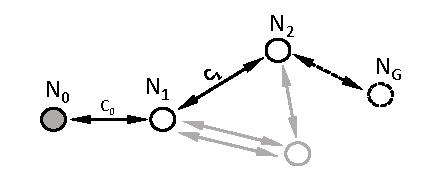
\includegraphics[width=0.99\linewidth]{img/measurement-topology.pdf}
      \caption{Measurement topology}
      \label{fig:measurement-topology}
\end{figure}

Once the funding transaction has completed (after the usual time to ensure Bitcoin consensus), 
$N_0$ starts measuring the capacity $\lambda_{1}$ by issuing a payment of $\lambda_t$, target capacity, 
to a \textit{ghost} node $N_G$.
This ghost node is a non-existent node, for which we generate a (non-existent) channel $C_{G}$ with a random identifier.
As the Lightning routing system is not aware of the ghost node, we request the routing system a route for $N_2$, 
and we modify the route to append the information corresponding to the last hop to $N_G$.
Thus, the resulting payment request, issued with a \texttt{sendtoroute} Lightning command, has a route $C_{0} \rightarrow C_1 \rightarrow C_{G}$. 
As neither $N_0$ nor $N_1$ validate the path with their routing information, the payment request is forwarded as long as enough capacity exits. 
However, when the request arrives to $N_2$, this node discards it, as it certainly knows there is no such node connected to it. 
Then the transaction is aborted, and an informative message is sent back to $N_0$.
Upon the reception of this message, we can deduce that $\lambda_t \leq \lambda_{0}$ and (more important to us) $\lambda_t \leq \lambda_{1}$, the channel to measure.
On the other hand, if $\lambda_t > \lambda_{1}$, then $N_1$ responds with a message indicating that there is not enough capacity in $C_1$, and also aborting the transference. 
In any of those cases, no hash-lock contracts are established, as they are only created from the payment receiver, in the direction to the issuer (would be created from $N_G$ to $N_2$, etc.), so no funds are blocked. 
Besides, as the computation requirements for this operation of checking and aborting are very low, the whole process is generally completed in less than a second. \ed{check!}

With the procedure described in the paragraph above we can test whether $\lambda_t \leq \lambda_{1}$. Let us call this procedure \textsc{EnoughCapacity}.
Then, we have that \textsc{EnoughCapacity}$(\lambda_t)=\mathit{True}$ if and only if $\lambda_t \leq \lambda_{1}$. 
We can use this procedure to devise the following strategy to obtain lower and upper bounds for the actual capacity of a channel $C_{1}$, as follows:
We start by assigning to $\lambda_t$ the initial target capacity advertised by the routing system, $\Lambda$, and we execute \textsc{EnoughCapacity}$(\lambda_t)$. If it returns $\mathit{True}$ (i.e., if the payment arrives to $N_2$), then we infer that the channel has the initial capacity.
%\footnote{We further check that there is no additional capacity to the advertised one by executing \textsc{EnoughCapacity} with $\lambda_t = \Lambda_{1} + \epsilon$, with $\epsilon$ a small value.} 
If it returns $\mathit{False}$ (the payment fails when arriving to $N_1$), then we move on checking another special case: whether the channel has no capacity left. To do so, we set $\lambda_t = \epsilon$ for a very small $\epsilon>0$ (since setting $\lambda_t = 0$ is not an option), and execute the procedure \textsc{EnoughCapacity}$(\lambda_t)$. If neither the capacity is the declared one, nor the channel is empty, 
we look for an intermediate capacity by an iterative binary search. 
The number of iterations of this loop is limited to $K$ (then, considering the test for the funding capacity and zero capacity, leads to a maximum number of payment requests per channel of $K+2$).
% For this, we perform an initial search to identify the order of magnitude of the current value, 
% by executing the procedure \texttt{EnoughCapacity} for $\Lambda_{1,2} / F^n$, with $F$ being a downscaling factor, 
% for $n: 1, 2, \ddots$, until a positive indication is reported.
% Then we execute a binary search that updates the maximum and minimum values observed so far. 
The result of the process is an estimation of the value for the actual capacity of the channel. 
We formalize the approach in Algorithm~\ref{alg:actual-capacity}.
% Note that the error can be expressed as $\frac{\lambda_{max} - \lambda_{min}}{2} = \Lambda 2^{-(K+1)}$}
The absolute error in the estimation made by the algorithm is $\epsilon$ for extreme values (either $\Lambda$ o 0 capacities), 
or $\Lambda \, 2^{-(K+1)}$ for the rest of the values, as resulting from a binary search. 
Therefore to obtain higher precision, higher values of $K$ can be used.

\begin{algorithm}
    \begin{algorithmic}[1]
    \Procedure{EstimateCapacity}{$C_{1}$, $K$}
    
    \State $\Lambda$ := \Call{GetFundingCapacity}{$C_{1}$}
    % \Comment{test initial capacity}
    \If{\Call{EnoughCapacity}{$\Lambda$}}
        % REMOVED CHECK FOR HIGHER CAPACITY: we observed some values for this
            % \If{not \Call{EnoughCapacity}{$\Lambda + \epsilon$}}  \Comment{Capacity is larger than advertised}
            %     \State return $\Lambda + \epsilon$
            % \Else
                \State return $\Lambda$
            % \EndIf
    \EndIf
    %\Comment{Test 0 capacity}
    \If{! \Call{EnoughCapacity}{$\epsilon$}}
        \State return 0
    \EndIf
    
    \State
    \State $\lambda_t$ := $\Lambda / 2$
    \State $\lambda_{max}$ := $\Lambda$
    \State $\lambda_{min}$ := 0
    \State counter :=0    
    \While {counter $< K$}
        \If{\Call{EnoughCapacity}{$\lambda_t$}}
        \State $\lambda_{min}$ := $\lambda_t$
        \State $\lambda_t$ := $\frac{\lambda_{min} + \lambda_{max}}{2}$
        \Else
            \State $\lambda_{max}$ := $\lambda_t$
            \State $\lambda_{t}$ := $\frac{\lambda_{min} + \lambda_{max}}{2}$
        \EndIf
        \State counter := counter + 1
    \EndWhile 
    

    \State return $\frac{\lambda_{min} + \lambda_{max}}{2}$
    \EndProcedure
    \end{algorithmic}
    \caption{Estimate $\lambda_{1}$ in a maximum of $K+2$ iterations with error $E = \Lambda \, 2^{-(K+1)}$ }
\label{alg:actual-capacity}
\end{algorithm}

Observe that, so far, we have not discussed the impact on the measurement of the node initially funding the channel (either $N_1$ or $N_2$).
% We have reasoned the capacity estimation procedure for the case $N_0$ connects to $N_1$ and measures
% a channel funded by $N_1$, i.e., measures $C_{1}$.
% It is straightforward to extend the procedure to the case, in which the channel was funded by $N_2$ (i.e., it is $C_{2,1}$). 
The fact is that, regardless of the node initially funding the channel, the transactions performed over the channel may result in any balance combination of the two directions, as far as the sum does not exceed \ed{[EQUALS??]} the value of the initial funding transaction. 
%This occurs regardless of the node performing the funding transaction.
% So, we set as maximum value of the capacity to be $\Lambda_{2,1}$, and we perform the tests. 
% To make the resulting capacity value independent of the node performing the funding transaction (either $N_1$ or $N_2$), we perform the following normalization for the measured value, $\lambda_{1,2}$: 
% If $N_1$, the node to which the measurement node attaches, was the node performing the funding transaction, we provide the measured capacity, $\lambda_{1,2}$.
% Conversely, if $N_2$ was the node which provisioned the funds, we provide $\lambda_{2,1}$, computed as $\Lambda_{2,1} - \lambda_{1,2}$. 
% In this way, regardless the node performing the funding transaction, the capacity estimation of the channel is positive, equal to the funding transaction value if no payment has been made, and 0 if the whole funded value has been transferred to the other node.

Finally, we comment the impact the experiment may have on the nodes under scrutiny.
The first cost is the computation resources required to establish a connection between $N_0$ and $N_1$. 
$N_1$ needs to send all the routing information to $N_0$. This process takes \ed{[Can we measure the mean time since we request a connection to when the connection is established? ]} 
Later, the nodes negotiate the setup of the channel. We deem this cost to be negligible compared to the exchange of routing information.
The second costs are associated to each capacity probe operation. For this case, 
note that the resources of the channel are not altered by the measure, as no transaction is finally performed. 
Besides, there is no temporal block of the resources, as the hash-lock contracts are not even established.
Additionally, we set a limit on the number of operations that can be requested to a node, to 3 operations per minute. 
The total number of transfers to perform with a node are limited to $K + 2$ times the number of channels of the node.